\documentclass[tikz,border=2pt]{standalone}
\usepackage{amsmath,amssymb}
\usepackage{pgfplots}
\pgfplotsset{compat=1.18}

\begin{document}
% Mixture picture of the continuous LOTP: X | Y = y ~ Unif(0, y) (boxes of height 1/y), weighted
% by f_Y(y) = 2y, gives the marginal density f_X(x) = 2(1 - x).
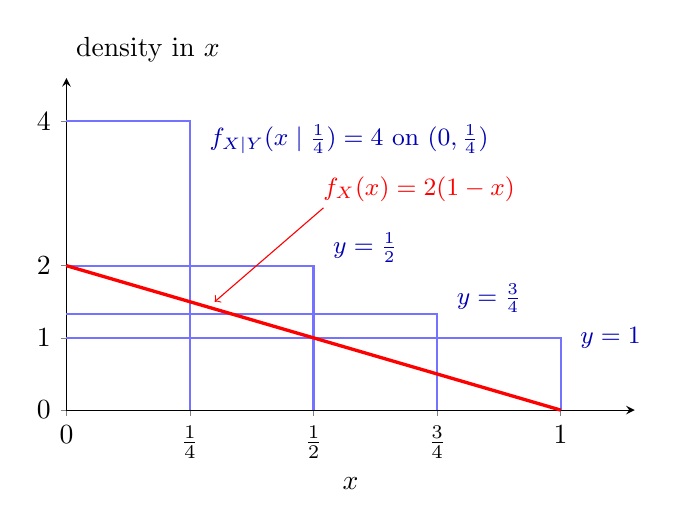
\begin{tikzpicture}
	\begin{axis}[
		axis lines=left, xmin=0, xmax=1.15, ymin=0, ymax=4.6,
		xtick={0,0.25,0.5,0.75,1}, xticklabels={$0$,$\tfrac14$,$\tfrac12$,$\tfrac34$,$1$}, ytick={0,1,2,4},
		xlabel={$x$}, ylabel={density in $x$}, ylabel style={rotate=-90, anchor=south west, at={(axis description cs:0,1.02)}},
		width=8.8cm, height=5.8cm, clip=false
		]
		\addplot[blue!55, thick] coordinates {(0,4) (0.25,4) (0.25,0)};
		\addplot[blue!55, thick] coordinates {(0,2) (0.5,2) (0.5,0)};
		\addplot[blue!55, thick] coordinates {(0,1.333) (0.75,1.333) (0.75,0)};
		\addplot[blue!55, thick] coordinates {(0,1) (1,1) (1,0)};
		\addplot[red, very thick, domain=0:1] {2*(1-x)};
		\node[blue!70!black, anchor=west, font=\small] at (axis cs:0.27,3.75) {$f_{X\mid Y}(x\mid\tfrac14)=4$ on $(0,\tfrac14)$};
		\node[blue!70!black, anchor=west, font=\small] at (axis cs:0.52,2.25) {$y=\tfrac12$};
		\node[blue!70!black, anchor=west, font=\small] at (axis cs:0.77,1.55) {$y=\tfrac34$};
		\node[blue!70!black, anchor=west, font=\small] at (axis cs:1.02,1) {$y=1$};
		\node[red, anchor=south west, font=\small] at (axis cs:0.5,2.75) {$f_X(x)=2(1-x)$};
		\draw[red, ->] (axis cs:0.52,2.8) -- (axis cs:0.3,1.5);
	\end{axis}
	
\end{tikzpicture}
\end{document}
